\label{sim_setup}

For this study, the Nelder Mead search algorithm parameters which were used can be seen in Table \ref{tab:nm_parameters}.
\begin{table}[!htb]
	\centering
	\caption{Nelder-Mead algorithm parameters}
	\label{tab:nm_parameters}
		\begin{tabular}{|c|c|} \hline 
			Parameter & Value \\ \hline
			$\alpha$ & 5.0 \\ \hline
			$\gamma$ & 10.0 \\ \hline
			$\beta$ & 0.5 \\ \hline
			$\sigma$ & 0.5 \\ \hline
		\end{tabular}
\end{table}
These parameters were chosen because they fell within the guidelines from the algorithm description and after trial and error produced the most efficient tuning \cite{nelder_1965}.

The starting values which were used as the starting point for the search algorithm can be seen in Table \ref{tab:starting_mat_prop_complete}.  These values were chosen based on the values which were found in literature for similar aluminum alloys.  The laser diameter which was chosen based on the measuring of a melt track width on a substrate. 
\begin{table}[!htb]
	\centering
	\caption{Material properties found in literature}
	\label{tab:starting_mat_prop_complete}
		\begin{tabular}{|c|c|c|c|} \hline 
			Property & Material Temp. & Value & Ref. \\ \hline
			Laser absorption & 880\degree C & 15.0\% & \cite{boyden_temperature_2006} \\ \hline
			Laser absorption & 922\degree C & 30.0\% & \cite{boyden_temperature_2006} \\ \hline
			Thermal conductivity & 922\degree C & 88.8 $\frac{W}{mK}$ & \cite{leitner_thermophysical_2017}\\ \hline
			Thermal conductivity & 1491\degree C & 104.9 $\frac{W}{mK}$ & \cite{leitner_thermophysical_2017}\\ \hline
			Specific heat & 733\degree C & 1108.0 $\frac{J}{kgK}$ & \cite{leitner_thermophysical_2017}\\ \hline
			Laser diameter & & 1.6 mm & \\ \hline
		\end{tabular}
\end{table}

The experimental setup which was used was a simple laser scanning of the surface of a substrate, as shown in Figure \ref{fig:melt_validation_example}, with the parameters shown in Table \ref{tab:exp_constants}.  This was chosen in order to simplify the experiment.  This setup removes the complexity associated with adding material including the rate of material addition, molten metal flow parameters and acceleration effect associated with turning during deposits.
\begin{figure}[!htb]
	\centering
	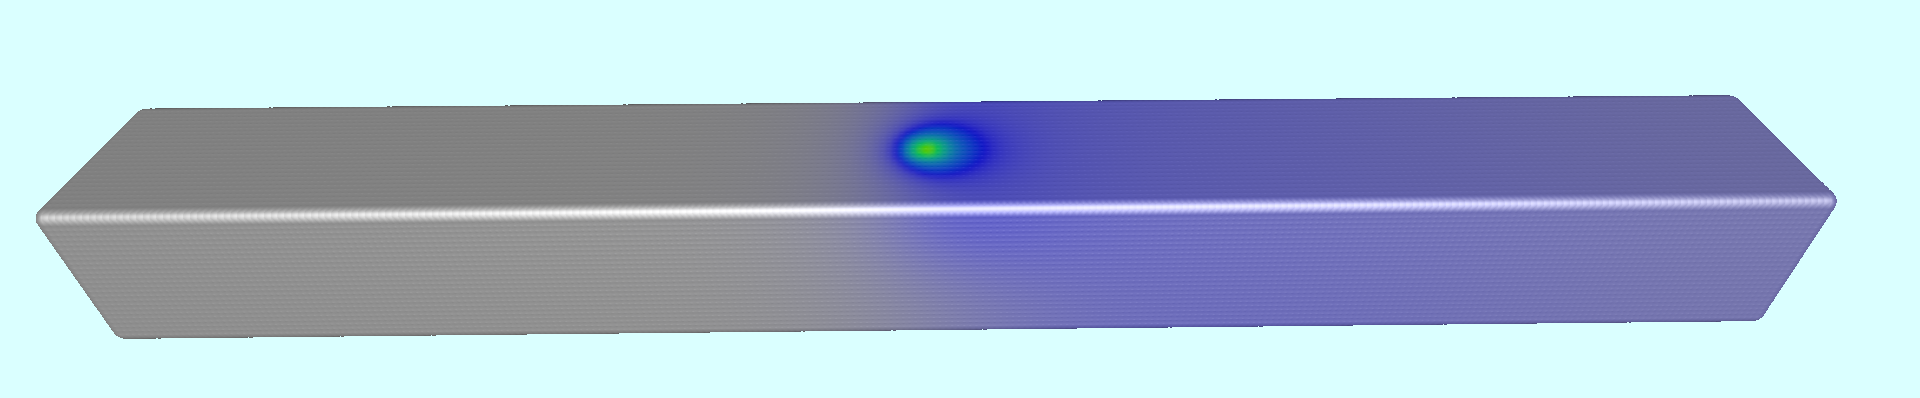
\includegraphics[width=0.75\textwidth]{melt_validation_example}
	\caption{Example of simulation setup used to determine melt track size}
	\label{fig:melt_validation_example}
\end{figure}
\begin{table}[!htb]
	\centering
	\caption{Experimental constants used in tuning experiments}
	\label{tab:exp_constants}
	\begin{tabular}{|l|l|} \hline
		Parameter & Value \\ \hline
% 			Material & NEED TO LOOK UP \\ \hline
		Resolution & 100 $\mu m$ \\ \hline
		Laser Power & 1,750 W \\ \hline
		Laser Scan Speed & 1143 mm/min \\ \hline
		Laser Profile & Top Hat \\ \hline
		Scan Length & 77 mm \\ \hline
		Substrate dimensions & 82 mm x 8 mm x 8 mm \\ \hline
	\end{tabular}
\end{table}


